% Restrained serif typeset (Libertinus via fontspec/unicode-math), small-caps section
% headings, hairline rules, one restrained teal-blue accent.
\documentclass[11pt]{article}

\usepackage{amsmath}
\usepackage{amsthm}
\usepackage{mathtools}
\allowdisplaybreaks

\usepackage{libertinus}   % Serif + Sans + Math + Mono via fontspec/unicode-math (XeTeX/tectonic-native; fixes the T1 libertinust1math glyph bug that mis-rendered % ~ approx times primes)

\usepackage[protrusion=true,expansion=false,final]{microtype}

\usepackage[letterpaper,top=1.2in,bottom=1.25in,left=1.5in,right=1.5in,
            headheight=15pt,headsep=15pt,footskip=26pt]{geometry}

\usepackage{xcolor}
\usepackage{graphicx}
\graphicspath{{../figures/}{figures/}}
\usepackage{booktabs}
\usepackage{array}
\usepackage{tabularx}
\usepackage{caption}
\usepackage{enumitem}
\usepackage{etoolbox}

\usepackage[nobottomtitles*]{titlesec}\renewcommand{\bottomtitlespace}{0.16\textheight}
\usepackage{titling}
\usepackage{fancyhdr}
\usepackage[framemethod=default]{mdframed}

\usepackage{hyperref}
\usepackage{xurl}

\definecolor{ink}{HTML}{1A1A1A}
\definecolor{accent}{HTML}{1F5066}
\definecolor{rulecol}{HTML}{343434}
\definecolor{subtle}{HTML}{6B7280}
\definecolor{sigbg}{HTML}{F4F6F7}

\hypersetup{colorlinks=true,linkcolor=accent,citecolor=accent,urlcolor=accent,
  filecolor=accent,breaklinks=true,bookmarksnumbered=false,
  pdftitle={Canonical self in cryptic cancer-epitope catalogues and the class-decoy ledger needed to verify non-canonical antigen claims},pdfauthor={Rom Jan},
  pdfsubject={Preprint}}
\urlstyle{same}

\setcounter{secnumdepth}{0}
\linespread{1.07}\frenchspacing\raggedbottom
\setlength{\parindent}{1.2em}
\widowpenalty=10000\clubpenalty=10000
\emergencystretch=1.6em \tolerance=1400 \hbadness=1400
\lefthyphenmin=3 \righthyphenmin=3   % no 2-letter hyphen fragments (bi-/de-/se-/re-)
\hyphenation{alt-ORF Cryptic-Protein-DB cancer}  % keep technical terms / the scare-quoted "cancer" intact
\setlist{itemsep=2pt,topsep=4pt,parsep=0pt}
\renewcommand{\arraystretch}{1.2}

\titleformat{\section}{\normalfont\large\bfseries\scshape\color{ink}}{}{0pt}{}%
  [\vspace{2pt}{\color{rulecol}\titlerule[0.4pt]}]
\titleformat{\subsection}{\normalfont\normalsize\itshape\color{ink}}{}{0pt}{}
\titlespacing*{\section}{0pt}{1.6\baselineskip}{0.5\baselineskip}
\titlespacing*{\subsection}{0pt}{1.0\baselineskip}{0.25\baselineskip}

\captionsetup{font=small,labelfont={sc,bf},labelsep=period,
  justification=justified,singlelinecheck=false,skip=7pt}

\newtheoremstyle{prep}{0.9\topsep}{0.9\topsep}{\itshape}{0pt}%
  {\scshape\bfseries}{.}{0.5em}{}
\theoremstyle{prep}
\newtheorem{proposition}{Proposition}
\renewcommand\qedsymbol{\textcolor{accent}{\rule[-0.02em]{0.55em}{0.55em}}}

\renewenvironment{abstract}{%
  \vspace{0.4em}\noindent{\color{rulecol}\rule{\linewidth}{0.4pt}}\par
  \vspace{0.7em}\centerline{\normalsize\scshape\color{ink}Abstract}\par\vspace{0.5em}%
  \begingroup\small\setlength{\leftskip}{1.9em}\setlength{\rightskip}{1.9em}%
  \setlength{\parindent}{0pt}\noindent\ignorespaces}{%
  \par\endgroup\vspace{0.7em}\noindent{\color{rulecol}\rule{\linewidth}{0.4pt}}\par\vspace{0.3em}}

% significance: unboxed, discreet small-caps run-in label in the body ink (no box/color)
\newenvironment{significance}{\par\addvspace{0.3em}\small\noindent
  {\scshape\bfseries Significance.}\enspace\ignorespaces}{\par\addvspace{0.55em}\normalsize}

\AtBeginEnvironment{thebibliography}{\footnotesize\setlength{\itemsep}{2.5pt}}
\newcolumntype{L}{>{\raggedright\arraybackslash}X}

\newcommand{\clsN}{\mathrm{N}}\newcommand{\clsC}{\mathrm{C}}
\newcommand{\TN}{T_{\clsN}}\newcommand{\TC}{T_{\clsC}}
\newcommand{\DN}{D_{\clsN}}\newcommand{\DC}{D_{\clsC}}
\newcommand{\VN}{V_{\clsN}}\newcommand{\VC}{V_{\clsC}}
\newcommand{\thn}{\theta_{\clsN}}\newcommand{\thc}{\theta_{\clsC}}
\newcommand{\thnhat}{\hat{\theta}_{\clsN}}
\newcommand{\SetN}{\Theta_{\clsN}}
\newcommand{\rhoeff}{\rho_{\mathrm{eff}}}\newcommand{\rhoglob}{\rho_{\mathrm{global}}}
\newcommand{\muN}{\mu_{\clsN}}\newcommand{\muC}{\mu_{\clsC}}
\newcommand{\msN}{m_{s\clsN}}\newcommand{\msC}{m_{s\clsC}}
\newcommand{\pisN}{\pi_{s\clsN}}\newcommand{\pisC}{\pi_{s\clsC}}
\newcommand{\E}{\mathbb{E}}
\DeclareMathOperator{\SE}{SE}
\DeclareMathOperator{\Poisson}{Poisson}
\newcommand{\Mlo}{m^{-}}\newcommand{\Mhi}{m^{+}}
\newcommand{\Glo}{g^{-}}\newcommand{\Ghi}{g^{+}}
\newcommand{\Slo}{s^{-}}\newcommand{\Shi}{s^{+}}

\setlength{\droptitle}{-2.4em}
\pretitle{\begin{center}\bfseries\LARGE\color{ink}\linespread{1.12}\selectfont}
\posttitle{\par\end{center}\vspace{0.4em}}
\preauthor{\begin{center}\large\color{ink}}
\postauthor{\par\end{center}}
\predate{\begin{center}\small\itshape\color{subtle}}
\postdate{\par\end{center}\vspace{0.2em}}
\title{Canonical self in cryptic cancer-epitope catalogues and the class-decoy ledger needed to verify non-canonical antigen claims}
\author{Rom Jan\\[3pt]
  {\normalsize\upshape Independent Researcher}\\[2pt]
  {\footnotesize\upshape\color{subtle}\textsc{orcid}~\href{https://orcid.org/0009-0004-1015-1627}{0009-0004-1015-1627}\,\textbullet\,Correspondence: \href{mailto:romjacobjan2005@gmail.com}{romjacobjan2005@gmail.com}}}
\date{Preprint \textemdash\ July 2026 \textbullet\ all analyses use public data and are fully scripted and reproducible}

\pagestyle{fancy}\fancyhf{}\renewcommand{\headrulewidth}{0pt}
\fancyhead[L]{\footnotesize\scshape\color{subtle}Canonical self in cryptic cancer-epitope catalogues}
\fancyhead[R]{\footnotesize\scshape\color{subtle}R.\,Jan}
\fancyfoot[C]{\small\color{subtle}\thepage}
\fancypagestyle{plain}{\fancyhf{}\fancyfoot[C]{\small\color{subtle}\thepage}%
  \renewcommand{\headrulewidth}{0pt}}

\begin{document}
\maketitle\thispagestyle{plain}
\begin{abstract}
Non-canonical open reading frames (ncORFs) are increasingly reported as sources of tumor-specific HLA antigens, but their clinical reuse depends on whether each published claim stays checkable after publication. We audited \textbf{306{,}844 published non-canonical tumor-antigen claims} (180{,}650 unique peptides) from two flagship end-to-end cohorts and the two largest public cryptic-peptide atlases, scoring only evidence in the reported record. The largest measured defect is sequence-level. \textbf{56.3\% of catalogued cryptic ``cancer'' epitopes in IEAtlas are exact substrings of the canonical human proteome}: canonical \emph{self} by sequence. This cannot serve as evidence for the non-canonical, tumor-specific antigen claim the catalogue nominates it for, whatever ORF it is attributed to. The effect is class-resolved, not field-wide. Primary-cohort altORF/lncRNA peptides are clean ($\approx$0.2\%), pseudogene-derived claims inherit canonical parent sequences (37.1\%), and a clean atlas (CrypticProteinDB, 0.0\%) shows the rate is avoidable; of the genuinely non-canonical remainder, 9.1\% appear on normal tissue. Separately, of all 306{,}844 claims \textbf{none} carries a machine-readable per-claim evidence package, a \textbf{reusability} gap that even known-real MAGE/SSX antigens share and that downstream pipelines inherit when they treat a catalogue row as a validated target. This locates the problem in reporting, not biology. The gap is structural: from reported summary statistics the non-canonical class false-discovery rate is only \emph{set}-identified. The single field that closes it is the per-class accepted decoy count $\DN$, a ``class-decoy ledger,'' which makes future claims re-verifiable on the three reporting-addressable axes it reaches (translation, presentation, specificity); immunogenicity requires its own reusable assay report.
\end{abstract}

\begin{significance}
A clinically important class of cancer antigens is being nominated faster than it can be checked from the published record. We show that a majority of catalogued cryptic ``cancer'' epitopes in the largest public atlas are canonical by sequence, that the published record essentially never carries the per-claim evidence to re-verify a claim, and that the gap has a provable statistical core. We then give the minimal reporting standard, a class-decoy ledger, that closes the identifiability gap.
\end{significance}

\section{Introduction}

The human genome is translated far more broadly than its $\approx$20{,}000 canonical protein-coding genes. Ribosome profiling and mass-spectrometry immunopeptidomics have shown that non-canonical open reading frames (ncORFs), found in long non-coding RNAs, pseudogenes, $5'/3'$ untranslated regions, and alternative reading frames of coding genes, give rise to short peptides that are presented on human leukocyte antigen (HLA) class~I molecules and recognized by T~cells~\cite{r13}. Because these ``dark-proteome'' or ``cryptic'' peptides can be tumor-restricted, they have become a prominent candidate source of tumor-specific antigens for cancer vaccines and T-cell therapies, and the published catalogue of such claims now numbers in the hundreds of thousands~\cite{r14,r15}.

A genuine tumor antigen must clear a four-step chain: its source ORF must be genuinely translated; its peptide must be genuinely HLA-presented; the peptide must be tumor-specific (absent from normal presentation); and T cells must genuinely respond. As the field moves toward the clinic, one prerequisite question, to our knowledge unmeasured, is whether the claims already in the literature carry, \emph{per claim}, the evidence needed for an independent party to re-verify them along this chain. This is a question about the reusability of the published record, not about the underlying biology.

One link in that chain rests on a statistical control that is known to be fragile for this class of peptide. Non-canonical peptides are identified by searching tandem mass spectra against vastly inflated databases (multi-frame translations of non-coding transcripts, pseudogenes, ncORF catalogues), with the false-discovery rate (FDR) controlled by target-decoy competition~\cite{r6}. It is well established that a single \emph{global} FDR pooled over canonical and non-canonical candidates underestimates the true FDR of the non-canonical subclass: because that subclass is typically a small fraction ($<$1--5\%) of accepted identifications, a global threshold is excessively permissive for it~\cite{r4,r5,r10,r11}. This has been quantified for over a decade: a nominal 1\% combined FDR was shown to correspond to a 36\% FDR for the novel-peptide class while the canonical class sat at 0.03\%~\cite{r19}. Recent immunopeptidomics pipelines adopt separate class-specific FDR for exactly this reason~\cite{r20}. The field's recommended remedies, class-specific (group) FDR and multistage search, concern \emph{how to compute} the subclass FDR when one holds the raw spectra and the per-class decoy counts~\cite{r5,r10,r11}. What has not been examined is the complementary, reproducibility-facing question: given only the statistics that papers actually \emph{report}, what can a reader independently conclude about a claim's class-specific FDR, and is that enough to re-verify the claim at all?

Here we make three contributions. \textbf{First}, we conduct what is, to our knowledge, the first systematic, leakage-controlled, public-data audit of the published non-canonical tumor-antigen record: 306{,}844 claims (180{,}650 unique peptides) from two flagship end-to-end cohorts and the two largest public cryptic-peptide atlases. We report two findings. (i)~A direct measurement: \textbf{56.3\% of catalogued cryptic ``cancer'' epitopes in IEAtlas are exact substrings of the canonical proteome} ($\approx$800$\times$ a composition-matched null), strongly class-dependent (pseudogene-ORF 37.1\%, altORF 0.2\%; a second atlas that applies a canonical filter is clean) and, to our knowledge, unquantified. (ii)~A re-verifiability result: scored exactly as reported on the four evidence axes, none of the claims carries reusable per-claim evidence on all four at once and only seven are auditable on all four; critically, known-real canonical cancer-testis antigens (MAGE/SSX) fail the identical bar, establishing this as a reporting and reusability gap rather than a statement about the biology. \textbf{Second}, we show the gap is structural, not incidental, by characterizing what the class-specific FDR can be from the reported statistics: it is only \emph{set}-identified, to the sharp interval $\bigl[0,\min(1,\alpha/(\TN/T))\bigr]$; the common upper ``budget'' bound is provably as tight as summary statistics allow; the quantity that governs the class decoy allocation at a threshold is a score-weighted \emph{effective} $\rho$ that can depart from the global candidate-space ratio (in a regime we characterize); and, propagated to the claim level, a calibrated per-claim truth probability is \textbf{not identifiable}; the honest output is a partial order over claims. \textbf{Third}, we give the minimal fix: a per-claim reporting standard that chiefly asks for the per-class decoy count $\DN$ on the claim's unit. It provably collapses the identifiability gap, together with a proposal for a neutral, leakage-controlled benchmark for the field.

Throughout, our claims concern the reporting and the statistics, never the biology: a reporting failure alone does not show that a peptide is unpresented or non-immunogenic, and the failure of the canonical controls under the same audit is our central guard against that misreading. Two narrower determinations do follow directly from what we measure: an exact canonical-substring match means the sequence and spectrum alone cannot establish a non-canonical origin, and a direct benign-ligandome match rules out strict absence from normal presentation, for that peptide sequence. All inputs are public and all analyses are scripted and openly reproducible (see Data and code availability).

\section{Results I. The audit: sequence non-novelty, specificity, and \mbox{re-verifiability}}

\subsection{A four-axis, as-reported audit of 306,844 published claims, stratified by resource type}
We assembled 306{,}844 published non-canonical tumor-antigen claims (180{,}650 unique peptides) from two flagship end-to-end immunopeptidomics cohorts, ovarian~\cite{r1} and hepatocellular carcinoma~\cite{r2}, together with the two largest public cryptic-peptide resources, IEAtlas (293{,}222 cancer epitopes) and CrypticProteinDB (9{,}101). These are different kinds of object, and we keep the strata separate throughout: a cohort paper \emph{could in principle} report a complete per-claim evidence package, whereas an atlas/catalogue record was never built to carry one. Each claim was scored, exactly as the source reports it, on four independent evidence axes: (i)~\emph{source-ORF translation} (is the ORF plausibly translated: Ribo-seq periodicity or the protein-existence consensus bar, applied to the ORF and not to the single ligand); (ii)~\emph{HLA presentation} (an eluted 8--12-mer with an assigned allele); (iii)~\emph{tumor specificity} (checked against a broad normal panel); and (iv)~\emph{immunogenicity} (an autologous or HLA-matched human T-cell response). A claim is a \emph{strict survivor} only if it strict-passes all four; anything the source leaves underspecified is labelled \emph{unverifiable} rather than failed. The auditor never recomputes FDR from spectra; it scores the evidence papers actually publish (Methods). We report two distinct findings: a direct, positive \emph{measurement} of sequence non-novelty, and a measurement of \emph{re-verifiability}, whether the reported record carries a reusable per-claim evidence package.

\subsection{More than half of catalogued cryptic ``cancer'' epitopes are canonical by sequence}
The first finding is a positive, \emph{measured} rate and, to our knowledge, the first time it has been quantified for these widely reused resources against the field's own sequence-novelty bar. Cross-referencing IEAtlas's own cancer epitope list against the canonical human proteome, \textbf{56.3\% (98{,}193/174{,}465)} of catalogued cryptic ``cancer'' epitopes are \emph{exact substrings of canonical proteins} and are therefore canonical \emph{self} by sequence (an identical sequence yields an identical spectrum), whatever ORF they are attributed to. This is \textbf{$\approx$800$\times$ a composition-matched shuffle null} (Fig.~\ref{fig:floors}), so the overlap is structural, not short-peptide coincidence. Nor is it an artifact of peptide length: restricting to the canonical HLA-I window (8--11mers) the rate is \textbf{53.9\% (67{,}852/125{,}999)}, and it rises monotonically with length (46.2\% at 8mer to 58.1\% at 11mer, 62.6\% beyond), as expected, since a longer exact canonical substring is stronger, not weaker, evidence of canonical origin. The rate is also stable under I/L collapse. Leucine and isoleucine are isobaric (113.084~Da) and MS-indistinguishable in standard fragmentation, so we additionally test each substring match allowing I$\leftrightarrow$L substitution: \textbf{56.5\% (98{,}546/174{,}465)}, a 0.2-percentage-point shift, confirming the headline rate is not an artifact of assuming a specific Leu/Ile assignment. Mechanistically these are predominantly \textbf{in-frame alternative ORFs of coding genes}. 88.8\% of the canonical-self epitopes are exact substrings of the canonical protein of \emph{their own annotated gene} (e.g.,\ the IEAtlas ORF \texttt{RBM47\_223aa} $\to$ RBM47), whereas the out-of-frame remainder that is \emph{not} canonical-self maps to its own gene's canonical protein in \textbf{0.0\%} of cases, an internal negative control confirming the substring test does not match spuriously (\texttt{src/darkproteome/ieatlas\_frame\_audit.py}). We use ``canonical self'' strictly as a \emph{sequence / MS-origin} criterion: an exact canonical-proteome substring is not sequence-novel, and the spectrum alone cannot establish a non-canonical origin. This is not a claim that the source ORF is untranslated. But the sequence alone cannot support the non-canonical, tumor-specific claim built on it, because the T-cell receptor and the mass spectrometer both read the sequence, not the locus. That non-canonical sets can harbour canonical sequences, and that pseudogene peptides are frequently identical to their parent protein, is recognised, and canonical-subtraction is a real, adoptable safeguard: CrypticProteinDB's own protein-level BLASTP canonical-exclusion filter (below) is a concrete, already-implemented example~\cite{r15}. A related large-scale non-canonical proteome/immunopeptidome study resolves ambiguous ORF assignment by priority-mapping (start-codon confidence, Kozak motif, transcript expression) but does not report a canonical-sequence overlap rate~\cite{r24}; what has not been reported is \emph{how large the rate is} in these catalogues. A complementary RNA-space approach, BamQuery, exhaustively enumerates the genomic regions capable of encoding a peptide and quantifies their expression in malignant and benign RNA-sequencing data; it addresses multi-locus origin attribution and RNA-level specificity rather than canonical-sequence exclusion~\cite{r28}.

It is strongly \textbf{class-resolved}, not uniform (Fig.~\ref{fig:floors}): in the primary cohorts, altORF and lncRNA-ORF peptides are essentially never canonical substrings (Raja altORF 0.2\%, 5/2{,}592; a composition-matched null gives $\approx$1$\times$, i.e.,\ no enrichment; these are genuinely non-canonical). This is not in tension with the 88.8\% in-frame figure above: Raja's altORF class is defined as \emph{out-of-frame} ORFs within a coding gene body, whereas IEAtlas's canonical-self burden is concentrated specifically in \emph{in-frame} ORFs of coding genes. It is the same frame distinction, not a contradiction between ``altORF'' classes, so the contamination has a precise mechanistic locus rather than being a property of altORFs generally. Pseudogene-ORF peptides, by contrast, carry an intrinsic risk of this failure, realized at 37.1\% (43/116) in the HCC cohort, each an exact substring of its parent canonical gene (e.g.,\ RPS3AP12 $\to$ RPS3A), a consequence of pseudogene biology, not negligence, that renders the peptide MS-unfalsifiable as pseudogene-derived rather than parent-derived. The risk is avoidable by upstream filtering, not absent in careful studies: Raja's own pseudogene-ORF claims are observed clean at 0/98 (Raja's stated filter excludes transcript biotypes protein\_coding/IG\_C/IG\_V, not a canonical-substring check specifically, so whether the 0/98 reflects a deliberate additional step or is incidental to their pipeline is not established by their reported methods). HCC's pseudogene-ORF claims were not clean, so the same biological hazard reached the published claim set regardless. The canonical-self burden is thus concentrated in the aggregator atlas and in the pseudogene class; the primary-cohort altORF/lncRNA peptides are clean. Critically, it is \textbf{resource-specific and avoidable, not intrinsic to cryptic-peptide catalogues}: at a comparable peptide-length profile, CrypticProteinDB carries \textbf{0.0\% (1/3{,}774)} canonical-self peptides versus IEAtlas's 56.3\%. IEAtlas's own methods~\cite{r14} report a combined PSM-level search against both the ncORF library and the canonical UniProt/Swiss-Prot proteome (FDR 0.05, no protein FDR), retaining epitopes by ORF-source label. An exact canonical substring yields an identical theoretical spectrum, so this PSM-level competition has nothing to discriminate on and cannot remove such a peptide, unlike CrypticProteinDB's additional protein-level canonical-alignment filter (BLASTP, E$<$0.01) applied before cataloguing, making CrypticProteinDB a clean negative control for the substring test.

Note the nulls differ by stratum: the $\approx$800-fold enrichment is an atlas-level statement, whereas the per-cohort altORF enrichment is $\approx$1$\times$. These four resources are not independent corroborations, and should not be read as such: IEAtlas aggregates public immunopeptidome deposits that include both cohorts, and 45 of the 48 cohort canonical-self peptides (Raja's 5 + HCC's 43) are already present in IEAtlas's own list. More broadly, across all ORF classes (not just canonical-self peptides), 823 peptides overlap in total between \{cohorts, CrypticProteinDB\} and IEAtlas (743 of all cohort peptides of any class; 80 of CrypticProteinDB's). The 56.3\% and 37.1\% figures are thus substantially overlapping measurements of the same underlying peptides, not separate confirmations across resources. Each remains individually correct over its own stated denominator, but the four-resource framing should be read as ORF-class-resolved slices of a largely shared corpus, not four independent measurements.

\subsection{A measurable tumour-specificity floor}
Among the genuinely non-canonical remainder (after removing the canonical-self peptides), \textbf{9.1\% (6{,}976/76{,}272)} appear in IEAtlas's \emph{own} normal-tissue epitope list, and nearly two-thirds of those map to a critical normal organ (brain/heart/liver/lung/kidney), a direct on-target/off-tumour signal that any pipeline reusing these atlases as a tumour-antigen source inherits. As a positive control, \textbf{16.3\% (15{,}960/98{,}193)} of IEAtlas's own canonical-self epitopes are independently re-detected on normal tissue by the HLA Ligand Atlas~\cite{r12}, 55.7\% of those on a critical organ. For the canonical-self pseudogene peptides specifically, an independent normal reference (the HLA Ligand Atlas~\cite{r12} benign HLA-I ligandome) directly observes 16 of 43 on normal tissue, a hard, finite-sampling-conservative floor on non-specificity. Separately, normal-tissue expression (GTEx v8) of the canonical parent gene itself is measured, not assumed, for all 43. Each is broadly expressed (median breadth: all 54 tissues), a specificity \emph{concern} at the RNA-expression level, not a presentation-level confirmation. Together, the non-novelty floor and this parent-gene expression signal flag all 37\% (43/116) of the HCC pseudogene ``antigen'' claims with at least the RNA-level concern; 16 of those 43 additionally carry the stronger, presentation-level confirmation of direct observation on the benign ligandome itself. A parallel gene-level screen extends to the lncRNA-ORF class at GTEx ENSG resolution: broad normal-tissue parent-gene expression (median $\ge$1~TPM in all 54 tissues) was observed for 0/93 HCC lncRNA-ORF claims versus 64/157 (40.8\%) Raja claims, localizing this RNA-level specificity concern to the Raja claim set; as above, this gene-level screen does not establish normal-tissue peptide presentation or immunogenicity.

\begin{figure}[tbp]\centering
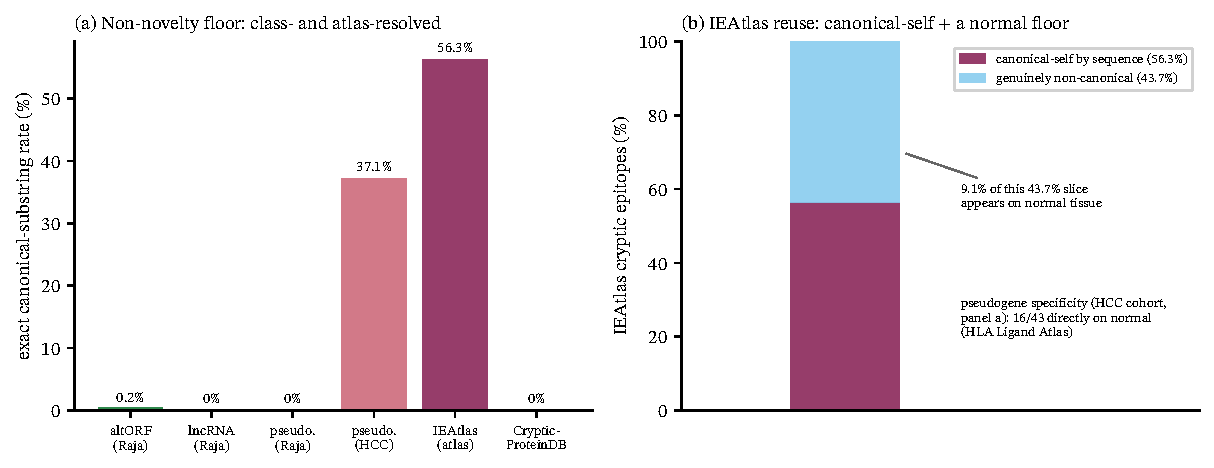
\includegraphics[width=\linewidth]{fig1_floors}
\caption{\textbf{Non-novelty and inherited specificity floors.} (a)~Exact canonical-substring rate by ORF class and atlas: altORF/lncRNA and Raja pseudogene $\approx$0\%, HCC pseudogene-ORF 37.1\%, and the IEAtlas catalogue 56.3\% versus a clean CrypticProteinDB at 0.0\%. The clean atlas adds a protein-level canonical-alignment filter that IEAtlas's combined-database PSM-level search competition cannot replicate. (b)~Of IEAtlas cancer ``cryptic'' epitopes, 56.3\% are canonical-self by sequence; of the genuine remainder, 9.1\% appear on normal tissue. Separately, of the HCC cohort's own canonical-self pseudogene peptides (panel a), 16/43 are directly observed in the benign HLA Ligand Atlas.}
\label{fig:floors}
\end{figure}

\subsection{No published claim carries a reusable four-axis evidence package}
Turning from sequence to re-verifiability: of 306{,}844 claims, \textbf{none} strict-pass all four axes, and only \textbf{seven} carry enough reported evidence to be even \emph{decidable} on all four at once (Fig.~\ref{fig:audit}). This bar measures the \emph{machine-readable reusability of the reported record}, not whether an antigen is biologically real, and reusability is exactly the property a downstream pipeline depends on when it treats a catalogue row as a validated target. The gap holds across both strata, for different reasons: the atlas records were never built to carry a per-claim T-cell assay or allele call, while the end-to-end cohorts complete the chain in their figures and prose but not in reusable, per-claim form. Critically, the bar is not unfairly harsh. A panel of known-real canonical cancer-testis antigens (MAGE/SSX), scored through the identical pipeline, \textbf{also fails} (0 strict survivors, N=144). That a positive control fails is expected, and is the central point: it locates the problem in the \emph{form of the reporting} rather than the truth of the biology, and makes the remedy a reporting standard rather than a wave of corrections. The published path from ``a peptide was observed'' to ``a validated tumor antigen'' is rarely available in reusable, per-claim, machine-readable form. The bar is satisfiable by construction, not vacuous: a claim reported with the class-decoy ledger (Table~\ref{tab:ledger}), a per-class decoy count, an assigned allele, quantified translation evidence, and a queried normal-ligandome search space, would strict-pass the three reporting-addressable axes (translation, presentation, specificity). The immunogenicity axis additionally requires the T-cell assay itself to be reported in reusable form, which no reporting standard can manufacture on its own; a claim carrying both the ledger and a reusable assay result would strict-pass all four, and the gap is unmet reporting, not an impossible standard.

\subsection{Where the evidence package breaks down}
The 0\% survival is forced jointly by two independently-zero axes, source-ORF and immunogenicity, not by knob-twisting on one (Fig.~\ref{fig:audit}). Source-ORF translation rigour is reported, per claim, for $\approx$0\% of the corpus, and the immunogenicity axis is empty of machine-readable human positives; either alone forces the joint result to 0\%. The HLA-presentation axis compounds this further with its own allele-assignment cliff: 99.96\% of unique peptides (all but $\approx$80) carry no per-peptide HLA allele in reusable form. Across both cohorts the maximal \emph{reusable} human-validated set tops out at $\approx$40 peptides, each requiring humanised-mouse data or manual figure digitisation to recover. An escalating-leniency analysis confirms the result is structural: strict survivors remain 0 even after fully relaxing the source-ORF and allele requirements, and reach only 41 when an entire axis is dropped (Methods).

\begin{figure}[tbp]\centering
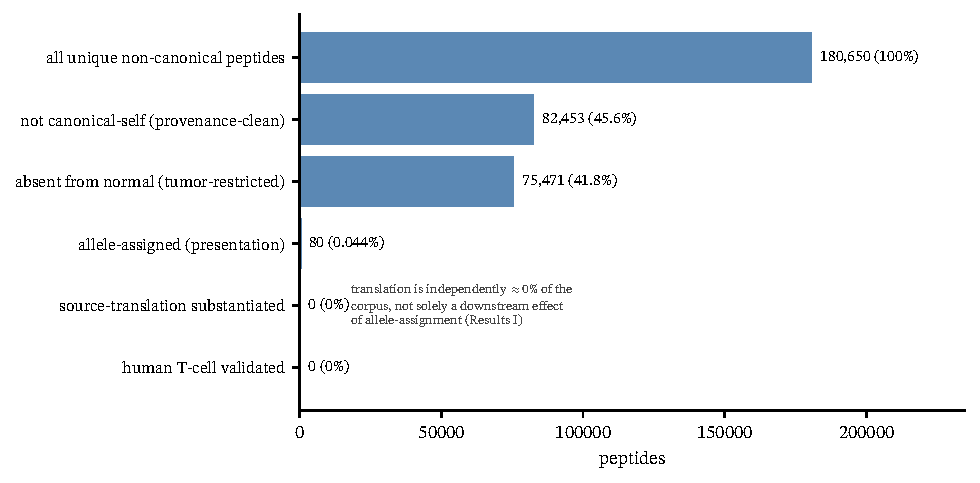
\includegraphics[width=\linewidth]{fig2_survivorship}
\caption{\textbf{The re-verifiability audit.} Of 306{,}844 published claims (180{,}650 unique peptides), none strict-pass all four evidence axes; the known-real canonical positive control (MAGE/SSX) collapses identically. Counts surviving each successive axis are shown on a linear scale so each step's true attrition is visually comparable; the two terminal zero-survivor counts are plotted at their true value ($x=0$). The first step's ratio (180{,}650$\to$82{,}453) is pooled across the full corpus and is a distinct measurement from the IEAtlas-specific 56.3\% canonical-self headline reported in Results I (different denominator and scope, not a discrepancy; Methods). The specificity step here (82{,}453$\to$75{,}471, 8.5\%) is pooled across all sources; it is a distinct measurement from the IEAtlas-specific 9.1\% normal-tissue rate reported in Results I, which uses IEAtlas's own genuinely-non-canonical remainder (76{,}272) as its denominator.}
\label{fig:audit}
\end{figure}

\section{Results II. The class-specific FDR is only set-identifiable; the per-claim truth is a partial order}

\subsection{The subsidy, made precise}
At a fixed acceptance threshold and a fixed statistical unit (PSM-, peptide-, or unique-peptide-level; mixing them invalidates what follows), let $\TN$, $\TC$ be the accepted target identifications in the non-canonical and canonical classes, $T=\TN+\TC$, and class fraction $f=\TN/T$. Let $\thn$, $\thc$ be the (unobserved) class false-discovery proportions and $q$ the global target-level false-discovery proportion on the same unit. By the law of total proportion,
\begin{equation}
q = f\,\thn + (1-f)\,\thc .
\label{eq:identity}
\end{equation}
A reported global FDR controlled at $\alpha$ gives only $q \le \alpha$; because the canonical class dominates the accepted set ($1-f \approx 1$), it absorbs most of the false budget and leaves $\thn$ nearly free. This is the formal content of the established observation that a pooled FDR underestimates the rare class's FDR~\cite{r4,r5,r10,r11}.

\subsection{The class FDR is set-identified, and the budget bound is as tight as the data allow}
Solving the identity for $\thn$ and letting the unobserved $\thc$ range over $[0,1]$ gives the \textbf{sharp identified set}
\begin{equation}
\SetN(q,f)=\left[\,\max\!\left(0,\ \frac{q-(1-f)}{f}\right),\ \ \min\!\left(1,\ \frac{q}{f}\right)\right].
\label{eq:idset}
\end{equation}
This is the same mixture-bound construction as the classical ecological-inference ``method of bounds''~\cite{r23}, applied here to a setting that literature never had: the class rate is \emph{directly observable} via the accepted decoy count (below), so the identifiability gap is a reporting omission rather than the permanent impossibility ecological inference confronts. When only $q \le \alpha$ is reported it widens to $\SetN=\bigl[0,\ \min(1,\alpha/f)\bigr]$. The upper endpoint is what we term the \emph{budget bound} (all false budget assigned to the non-canonical class). We prove it \textbf{sharp}: for any $\theta^{*}$ in the set, the implied canonical rate $\thc^{*}=(q-f\theta^{*})/(1-f)$ lies in $[0,1]$, and a law in which non-canonical targets are false at rate $\theta^{*}$ and canonical targets at rate $\thc^{*}$ reproduces the same reported $(q,f)$ (Methods, Prop.~\ref{prop:idset}). Two consequences: \textbf{(a)}~no estimator can tighten the budget bound from the reported summary statistics alone; it is the best possible. \textbf{(b)}~the lower endpoint is $0$. A global FDR statement forces no false discovery into the non-canonical class, so summary statistics can never show a class FDR is \emph{high}, only bound how high it could be.

For the ovarian cohort~\cite{r1} ($\alpha = 3\%$, PSM-level; $f$ below is on the same unit): the headline noncoding-cryptic subset is $<$1\% of accepted identifications ($f < \alpha$), so its class FDR set is $[0,1]$, entirely unconstrained by the reported 3\%. The broader cryptic class ($f = 4.4\text{--}7.1\%$) gives $\SetN=[\,0,\ 42\text{--}68\%]$, an upper bound 14--23$\times$ the reported global figure (Fig.~\ref{fig:theory}a). This bounds what the \emph{published statistics} support, not the realized class FDR, which direct re-searches with class-specific decoys have shown can in fact be large (e.g.,\ 36\% at a nominal 1\%~\cite{r19,r20}). That the realized value can be high yet remain invisible to the reported global figure is precisely the identifiability gap, not a claim that this cohort's realized class FDR is high.

\subsection{A diagnostic: the class split follows an \emph{effective} \texorpdfstring{$\rho$}{rho}, not the global candidate ratio}
One might predict the class split of false (decoy) discoveries from search-space sizes. Under a common null with per-spectrum top-hit competition, the expected accepted-decoy ratio is a \emph{threshold-weighted} average of per-spectrum class fractions,
\begin{equation}
\rhoeff(\tau) = \frac{\sum_s w_s\,\pisN}{\sum_s w_s\,\pisC},
\qquad w_s = 1-F(\tau)^{m_s},\quad \pi_{sg}=\frac{m_{sg}}{m_s}
\label{eq:rhoeff}
\end{equation}
(derivation in Methods), \textbf{not} the global ratio $\rhoglob=\sum_s \msN / \sum_s \msC$. The two can diverge arbitrarily (e.g.,\ one spectrum $(m_{\clsN},m_{\clsC})=(900,100)$ plus a hundred $(1,9)$ spectra give $\rhoglob = 1$ but $\rhoeff = 0.21$ at a per-candidate tail probability $t=1-F(\tau)=0.01$; the same construction gives $\rhoeff\approx0.96$ at $t=10^{-4}$ and $\rhoeff\approx0.12$ as $t\to1$, so the toy value is threshold-specific, not construction-intrinsic), and a direct simulation confirms the accepted $\DN/\DC$ tracks $\rhoeff$, not $\rhoglob$, as the threshold relaxes (Fig.~\ref{fig:theory}b, a separate, larger heterogeneous-population simulation, not the two-spectrum toy example above; Methods). We treat $\rhoeff$ as a diagnostic, not a measured quantity: the common-null assumption it requires is least secure exactly where $\rhoeff$ departs from $\rhoglob$ (non-tryptic cryptics plausibly have $F_{\clsN}\ne F_{\clsC}$), and in the stringent-threshold limit relevant to typical immunopeptidomics operating conditions $\rhoeff\to\rhoglob$. But the reported record does not establish which per-candidate tail probability $t$ a given cryptic search actually corresponds to, so whether a given cohort is sufficiently far into that limit is itself an empirical question, resolved only by the class-labelled decoy counts $\DN(\tau),\DC(\tau)$, absent from the reported record.

\begin{figure}[tbp]\centering
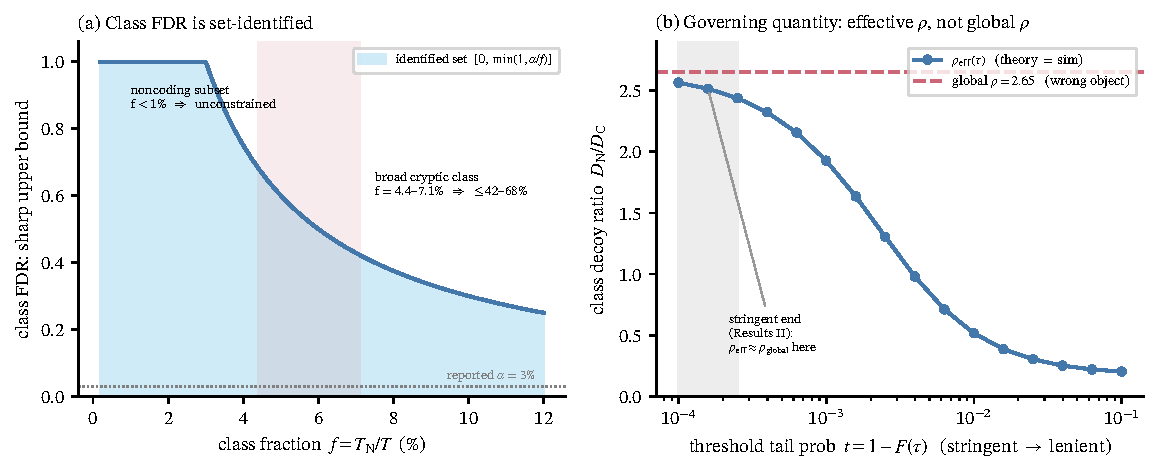
\includegraphics[width=\linewidth]{fig3_theory}
\caption{\textbf{The identifiability theory.} (a)~The class-specific FDR is only set-identified; the sharp upper bound is $\min(1,\alpha/f)$, giving $\le$42--68\% for the broad cryptic class ($f=4.4\text{--}7.1\%$) at the reported $\alpha=3\%$. (b)~A diagnostic: the class decoy split follows a threshold-weighted effective $\rho$, not the global candidate ratio: simulated $\DN/\DC$ tracks $\rhoeff(\tau)$ and drifts from $\rhoglob$ as the threshold relaxes; the shaded band marks this simulation's stringent end, where $\rhoeff\approx\rhoglob$ --- the limit Results II characterizes as typical for immunopeptidomics operating conditions, without establishing that any given cohort actually sits there.}
\label{fig:theory}
\end{figure}

\subsection{A single statistic collapses the uncertainty}
Both results point to one missing datum. The class FDR becomes \textbf{consistently estimable}, by the ordinary target-decoy estimate $\thnhat = (\DN+1)/\TN$~\cite{r6,r7,r25}, exactly when the per-class accepted decoy count $\DN$ is reported on the claim's unit and convention (equivalently, when the per-class decoy \emph{split} is recoverable, since the reported global FDR and class fraction fix the total); absent it, the class FDR is \textbf{not identifiable} from the published record (Methods, Prop.~\ref{prop:ident}); no alternative report identifies it without also determining $\DN$ (Methods, Cor.~\ref{cor:necessity}). $\DN$ is the single number that turns an unfalsifiable interval into a checkable estimate. We stress the scope of that claim: $\DN$ closes the \emph{reconstructibility} gap. It makes the class estimate \emph{computable}, but whether the estimate is well-\emph{calibrated} is a separate question, since the target-decoy equal-chance assumption can be fragile for the inflated, often non-tryptic cryptic search space; only an entrapment-based check settles it. The reporting standard below therefore asks for $\DN$ together with a matched entrapment result.

\subsection{Per-claim truth is an upper-bound ranking, not a probability}
Propagated to the object a reader ultimately wants, the probability a single claim is true, the set-identification has a sharp consequence. Lacking reusable immunogenicity evidence (Results~I), we bound \emph{presented-ligand} truth $Y = M\cdot G\cdot S$ (correctly-identified $\times$ genuinely non-canonical $\times$ tumor-specific), not full antigen truth. The three channels are coupled (search-space inflation ties $M$--$G$, pseudogene-parent identity ties $G$--$S$, detectability ties $M$--$S$), so the per-claim probability is not a product of marginals; the sharp Fr\'echet bounds (Methods) give
\begin{equation}
P(Y=1)\in\bigl[\,\max(0,\ \Mlo+\Glo+\Slo-2),\ \ \min(\Mhi,\Ghi,\Shi)\,\bigr].
\label{eq:frechet}
\end{equation}
The $M$-marginal lower bound is $1-\min(1,\alpha/f)$, which reaches $0$ only when $f\le\alpha$ (the headline noncoding-cryptic subset); more generally it is strictly positive (e.g.\ $0.32$--$0.58$ for the broader cryptic class). On the present data, though, every claim's \emph{joint} probability still has lower bound $0$. This is not because of the $M$-marginal, but because the non-novelty and specificity floors (Results~I) each independently reach a lower bound of $0$ for any single claim, and that alone collapses the Fr\'echet joint lower bound. So every such claim's probability is \textbf{not point-identified}. Claims are comparable only by their sharp \emph{upper} bound (a partial order) over claims not yet individually inspected beyond class membership. On our data a random Raja altORF claim has $P \le 0.998$ versus a random HCC pseudogene claim $P \le 0.629$ (the 37.1\% non-novelty floor) (Fig.~\ref{fig:partial}): a class-conditioned upper-bound ranking, not a calibrated per-claim probability. Once a specific claim's own indicators are observed they supersede the class-average marginal directly: an exact-canonical-substring claim collapses to $P = 0$ regardless of class, and a claim already confirmed non-canonical-self is bounded above its class average, not by it. Crucially, our three audit instruments \emph{are} the marginals of this object: the non-novelty floor is $1-\Ghi$, the normal-presentation floor is $1-\Shi$, and the class-FDR budget bound is the $M$-marginal. So the empirical audit (Results~I) and the identifiability theory are one construction, not two.

\begin{figure}[tbp]\centering
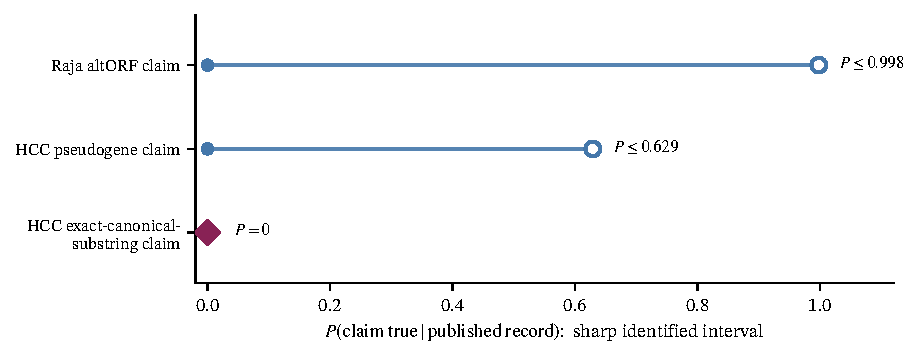
\includegraphics[width=0.82\linewidth]{fig4_partial_order}
\caption{\textbf{Per-claim truth is a partial order.} For a claim not yet individually inspected beyond class membership, truth admits only a sharp class-conditioned upper bound on $P(\text{true})$, not a point value: a random Raja altORF claim $P\le 0.998$, a random HCC pseudogene claim $P\le 0.629$. Once a claim's own status is observed that value collapses to a point instead: an exact-canonical-substring claim has $P=0$, regardless of class. Both non-degenerate intervals share the lower bound $0$, so the class-conditioned case is an upper-bound ranking, not set-dominance. Intervals are drawn open-capped at the upper bound (a bound, not a confirmed value); the filled diamond marks the point-identified $P=0$ case.}
\label{fig:partial}
\end{figure}

\subsection{Acting on an identified set: a triage rule}
The partial order has an operational reading. With each claim's truth probability bounded to a sharp identified interval $P(Y=1)\in[L,U]$ (Methods), a user selecting targets at a benefit/cost break-even $p^{*}=C/(B+C)$ can act by interval dominance: \textbf{reject} if $U < p^{*}$ (even the best compatible probability is too low), \textbf{accept} if $L \ge p^{*}$ (even the worst clears the bar), and otherwise treat the claim as \textbf{not identified}, collecting the one missing statistic (the per-class decoy count $\DN$ for the $M$-factor; a normal-ligandome search for the $S$-factor) rather than guessing a probability. Ranking the not-identified claims requires a stated risk posture (optimistic, by $U$; conservative, by $L$; minimax-regret weighs both): the reported record yields the \emph{set}, and the user chooses the rule~\cite{r18}. On the present data this rarely licenses acceptance, since class-FDR lower bounds are zero, so its value is a valid rejection/triage rule and a precise statement of which single measurement would change the decision.

\section{Results III. A reporting standard, a neutral benchmark, and its feasibility}

\subsection{A minimal reporting standard makes claims re-verifiable}
The identifiability results convert directly into a short, actionable reporting standard: a minimum-information \textbf{class-decoy ledger} that travels with each non-canonical antigen claim and supplies exactly the statistics that collapse the identified sets to checkable estimates (Table~\ref{tab:ledger}; reference implementation \texttt{class\_decoy\_ledger.py}). The single most important field is the \textbf{per-class accepted decoy count $\DN$}, on the same unit (PSM / peptide) and FDR convention as the claim; with it, the class FDR becomes the ordinary target-decoy estimate rather than an unfalsifiable interval. The remaining fields close the other axes: the class target counts and fraction ($\TN,\TC,f$); the FDR convention and unit, stated explicitly; the per-peptide HLA allele; machine-readable source-ORF translation evidence (periodicity or protein-level statistics) and the peptide's canonical-substring status; and, for tumor specificity, the normal-ligandome search space actually queried with its class-specific decoy counts. None of these requires new wet-lab experiments. The decoy and target counts, FDR convention, and unit already arise from the original search pipeline and are discarded at reporting time, not recomputed; the canonical-substring status and normal-ligandome query are additional computational checks on already-public sequence and reference data, not new assays --- and, per Results~I, are frequently \emph{not} already performed by the original analysis.

\subsection{A neutral, leakage-controlled benchmark}
A reporting standard fixes new claims but cannot, by itself, adjudicate the existing record or grow the missing ground truth. We therefore propose a neutral, openly governed benchmark for non-canonical tumor antigens, on the model of community benchmarks in adjacent fields where the party controlling the ground truth is distinct from those being evaluated (organizer $\ne$ competitor $\ne$ assessor). Two tiers follow the evidence: a \textbf{presentation tier}, buildable now from public data, scoring claims on the re-verifiable axes under one uniform class-specific-FDR pipeline; and a small \textbf{immunogenicity tier}, grown prospectively with time-separated or embargoed ground truth to prevent the circularity that would otherwise let a method be tuned on its own test set. The audit of Results~I is the natural seed. It defines the corpus, the axes, and the failure modes the benchmark must measure.

\subsection{The empirical check has adequate statistical power for one researcher}
The standard asks authors for $\DN$; for the already-published record, the same statistic is recoverable independently. The class-labelled decoy count $\DN(\tau)$ can be obtained by re-searching public raw spectra under a class-preserving target-decoy design, and an entrapment search~\cite{r8,r9} independently tests whether the target-decoy control is actually calibrated for the cryptic class. A power analysis shows the statistical precision is within reach of a single researcher on public data --- a distinct question from end-to-end operational cost, addressed separately: for an entrapment search at multiplicity $k$ over a class of $n$ accepted non-canonical discoveries with true FDR $\theta$, the estimate has standard error $\sqrt{\theta/(kn)}$, so for the ovarian cohort's headline class ($n \approx 311$) a single matched entrapment ($k = 1$) already resolves the class FDR to a 95\% half-width of $\approx$9 percentage points, enough to distinguish, e.g., a 40\% from a 70\% class FDR. This precision is governed by the absolute number of accepted non-canonical discoveries $n$, not by the class's vanishing fraction of the catalogue, so the rarity of the class is not itself an obstacle to estimating its FDR. The decisive comparison is then whether the measured ratio $\DN(\tau)/\DC(\tau)$ tracks $\rhoeff(\tau)$ or the global candidate ratio across thresholds. This is the test that converts the identifiability bound into a number. Philosopher's group-specific FDR filtering already implements the class-preserving step this re-analysis would need: it separates PSMs by class and computes the per-class accepted-decoy count at the point of filtering, then discards it --- Philosopher's own report command excludes decoy rows from every output file unless a user explicitly passes \texttt{-{}-decoys} (default \texttt{false}), so $\DN$ is unrecoverable even from the deposited PSM-level output~\cite{r26}. A recent immunopeptidomics study applies exactly this design to a canonical-vs-non-canonical split (protein-existence groups PE~1 and PE~4): its Methods state the resulting group-specific FDR threshold (0.03) repeatedly, but not the decoy count behind it~\cite{r27} --- the gap Table~\ref{tab:ledger} is built to close, already latent in the pipeline the field runs today. This re-analysis is the natural next study; it is not required for the present results, which stand on the published record and the identifiability theory.

\begin{table}[tbp]\centering
\caption{\textbf{The class-decoy ledger: a minimal per-claim reporting standard.} Each field is a quantity the original analysis already computes; reporting it makes the corresponding identified set checkable. All FDR fields are on one stated statistical unit (PSM / peptide / unique-peptide) and threshold.}
\label{tab:ledger}
\footnotesize\setlength{\extrarowheight}{3.5pt}
\begin{tabularx}{\textwidth}{@{}>{\raggedright\arraybackslash}p{0.42\textwidth}>{\raggedright\arraybackslash}X@{}}
\toprule
\textbf{Field to report (per claim)} & \textbf{What it makes re-verifiable} \\
\midrule
Statistical unit $+$ FDR convention ($D/T$, $(D{+}1)/T$, \ldots) & Makes every FDR figure interpretable; without it the class-FDR identity cannot be applied at all \\
Class target counts $\TN$, $\TC$ ($\Rightarrow$ fraction $f$) & Yields the sharp budget bound $\bigl[0,\min(1,\alpha/f)\bigr]$ \\
\textbf{Per-class accepted decoy count $\DN$} (same unit $+$ threshold) & \textbf{Collapses the class FDR to the target-decoy estimate $(\DN{+}1)/\TN$, the single highest-value field (computability)} \\
\emph{(paired)} a matched entrapment class-FDP check & Calibration: confirms the $(\DN{+}1)/\TN$ estimate is unbiased; target-decoy alone gives computability, not calibration \\
Per-peptide HLA allele & The presentation axis (resolves the allele-assignment cliff) \\
Source-ORF translation evidence (Ribo-seq periodicity \% or protein-level FDR $+$ $\ge$2 unique $\ge$9-aa peptides), machine-readable & The translation axis \\
Peptide canonical-substring status vs a named proteome version & The non-novelty floor (the $G$ factor) \\
Normal-ligandome search space queried $+$ its class-specific decoy counts & The specificity axis (the $S$ factor); distinguishes ``absent'' from ``not searched'' \\
\emph{(recommended)} per-spectrum candidate counts $\msN$, $\msC$ & Recovers the effective $\rho$; diagnoses the global-$\rho$ shortcut \\
\bottomrule
\end{tabularx}
\end{table}

\section{Discussion}

We set out to measure whether the published dark-proteome tumor-antigen record can be independently re-verified. We found, first, a concrete measured defect: \textbf{56.3\% of catalogued cryptic ``cancer'' epitopes in IEAtlas are canonical by sequence} ($\approx$800-fold over a composition-matched null, strongly class-dependent, and to our knowledge unquantified by any atlas), and, more broadly, that the record as reported essentially cannot be re-verified: of 306{,}844 claims, none carry reusable per-claim evidence across all four evidence axes, and known-real canonical antigens fail the same bar. The contribution of this work is to show that this is not merely uneven reporting but has a structural core. The class-specific false-discovery rate underwriting the presentation axis is only \emph{set}-identified from the statistics papers report; the common budget bound is provably the tightest such bound; the quantity that governs the class allocation at a threshold can be a threshold-weighted \emph{effective} $\rho$ rather than the global candidate ratio (in a regime we characterize); and, propagated to the claim level, a calibrated per-claim truth probability is not identifiable at all. The honest audit output is a partial order. A single reported statistic, the per-class decoy count $\DN$, collapses the central uncertainty.

That the canonical controls fail the same audit is the result's most important feature, not a caveat (Results~I): the remedy is accordingly a standard, not a wave of corrections. Our recommendation mirrors and extends the field's own reform trajectory: the HUPO/HPP~\cite{r17} and GENCODE Ribo-seq ORF~\cite{r16} reporting standards, entrapment-based assessment of FDR control~\cite{r8}, the established recognition that class-undiscriminated FDR underestimates rare-class error~\cite{r4,r5,r19}, and recent calls for verifiable FDR reporting more broadly~\cite{r21}. Concurrent work proposes general verifiable-FDR diagnostics, the scope, calibration, and stability of any reported FDR, with decoy-inclusive outputs for independent checking~\cite{r21}; our contribution is the complementary, \emph{class-specific} core: a proof that the non-canonical class FDR is unidentifiable from summary statistics without the per-class decoy count, and the single field ($\DN$) that closes it. Where prior work asks \emph{how to compute} a class-specific FDR from raw data~\cite{r5,r10,r11,r22}, we ask what a reader can conclude from the published \emph{summary statistics}, and answer it with a partial-identification analysis~\cite{r18} and a concrete class-decoy ledger that makes the needed quantities travel with the claim. The set-identification is not specific to immunopeptidomics: the same mixture identity bounds any rare relevant subclass's FDR from a pooled target-decoy threshold. Proteogenomics, rare post-translational modifications, and any setting where a global multiple-testing threshold is applied to a small relevant subset all qualify, so the contribution is the publication-record estimand (what a reader can identify from the summaries papers report) and the class-decoy ledger that closes it, not the elementary mixture algebra itself.

Several limitations bound the scope. The full four-axis chain is measured on the two cohorts that report it end to end; the atlas scale-up tests the generality of the reporting gap but not of the immunogenicity axis, whose reusable human ground truth is genuinely thin ($\approx$40 peptides, largely figure-locked). The identifiability results are statements about what the published record \emph{supports}; they neither assert nor deny that any specific antigen is real, nor do they by themselves determine presentation or immunogenicity from reporting completeness alone. Where the sequence and benign-ligandome audits directly measure a specific claim, those measurements do support the narrower, claim-level conclusions reported in Results~I and~II. Establishing the realized class FDR for a given study, and thereby testing empirically whether $\DN(\tau)/\DC(\tau)$ tracks the effective or the global $\rho$, requires re-analysis of raw spectra, which we show is feasible for one researcher on public data but leave to a dedicated study. Finally, the composition-matched null underlying the non-novelty enrichment is stochastic and is reported as a bound.

As non-canonical antigens move toward the clinic, the cost of a claim that cannot be re-verified rises. The fix we propose is cheap, a short class-decoy ledger of statistics the original analysis already computed, and it converts a class of claims that today cannot be independently checked into one that can be, on the three axes reporting alone can fix; the fourth, immunogenicity, still needs its own reusable assay report.

\section{Methods}

\subsection{Corpus assembly and statistical unit}
We assembled 306{,}844 claims (180{,}650 unique peptides): two end-to-end immunopeptidomics cohorts, ovarian~\cite{r1} and HCC~\cite{r2}, plus IEAtlas (293{,}222 cancer epitopes) and CrypticProteinDB (9{,}101; 8{,}879 cryptic immunopeptides $+$ 222 allele-resolved epitopes), with 144 canonical cancer-testis antigen claims (MAGE/SSX; 37 unique peptides) as a positive control. IEAtlas reanalyzes public immunopeptidome deposits and therefore overlaps the other resources at the peptide level (823 peptides shared between \{cohorts, CrypticProteinDB\} and IEAtlas: 743 cohort, 80 CrypticProteinDB; see Results~I for the reading this supports). Claims are deduplicated and stored in a 19-column contract (Supplement). Headline rates use resource-specific denominators, stated at each use: the 56.3\% canonical-self rate is over the 174{,}465 unique IEAtlas cancer peptides entering the substring test (the 293{,}222 catalogue rows after deduplication; the peptides range 8--25 residues, with no upper length filter), the 9.1\% normal-tissue rate is over the 76{,}272 genuinely non-canonical remainder, and 306{,}844\,/\,180{,}650 count claims / unique peptides across all resources. \textbf{Unit discipline:} every class-FDR quantity below is computed at one fixed statistical unit (PSM-, peptide-, or unique-peptide-level) and one acceptance threshold; mixing units (e.g.,\ PSM-level decoys against peptide-level claims) invalidates the identity in \S\,``Identified set''.

\subsection{Four-axis, as-reported scoring}
Each claim is scored on four axes with the field's standards: source-ORF translation (Ribo-seq $\ge$70\% periodicity \emph{or} the protein-existence consensus bar~\cite{r3}, applied to the ORF, never to a single 8--12-mer ligand); HLA presentation (eluted 8--12-mer with an assigned allele); tumor specificity (broad normal panel); immunogenicity (autologous/HLA-matched human T-cell assay). Underspecified fields are labelled \emph{unverifiable}, not failed. The auditor independently recomputes the consensus-bar verdict from raw fields. Robustness is assessed with an escalating-leniency ladder (Supplement): strict survivors remain 0 through relaxation of the source-ORF and allele requirements and reach 41 only when an entire axis is dropped. We do not report a Wilson confidence bound on the strict-survivor proportion as a generalization interval: claims share resources, studies, peptides, and reporting schemas, so the corpus is not an independent Bernoulli sample and no such bound would describe uncertainty over a superpopulation of published claims. As an independence-reference calculation only, not a claim of statistical validity, the two-sided 95\% Wilson upper endpoint is 0.0013\% for the audited claims and 2.6\% for the 144-claim canonical-control panel.

\subsection{Non-novelty floor}
A peptide that is an exact substring of the SwissProt (reviewed) human proteome is canonical-self by sequence (identical sequence $\Rightarrow$ identical spectrum). We compute exact and I/L-collapsed substring rates per ORF class, with a composition-matched shuffle null (seeded) and Wilson 95\% intervals; pseudogene parent genes are mapped from the \texttt{GN=} field. The shuffle-null enrichment multiplier is stochastic and reported as a bound ($\approx$800$\times$, i.e.,\ ${>}$\,several-hundred-fold).

\subsection{Specificity floor}
For canonical-substring peptides the correct normal reference is canonical-space: the HLA Ligand Atlas benign HLA-I ligandome. We test exact membership and map hits to tissue criticality. Absence from a finite atlas is treated as non-informative (a conservative floor), never as positive evidence of specificity.

\subsection{Class-specific FDR: identified set and identifiability}
Fix the unit and threshold, and \textbf{condition on the observed accepted counts} $\TN,\TC$ ($T=\TN+\TC$, $f=\TN/T$); let $\thn=\E[\VN/\TN]$, $\thc=\E[\VC/\TC]$ be the (conditional) class false-discovery proportions and $q=\E[(\VN+\VC)/T]$ the global one. Because $f$ is then fixed, $q = f\,\thn + (1-f)\,\thc$ holds exactly (Eq.~\ref{eq:identity}). We take a reported ``global FDR controlled at $\alpha$'' to mean the target-decoy estimate bounds the expected global FDP, $q \le \alpha$ (the standard, calibration-dependent reading).

\begin{proposition}[sharp identified set]\label{prop:idset}
The set of $\thn$ consistent with a reported $(q,f)$ and $\thc\in[0,1]$ is $\SetN(q,f)=\bigl[\max(0,(q-(1-f))/f),\ \min(1,q/f)\bigr]$, and every value is attained.
\end{proposition}
\begin{proof}
$\thn=(q-(1-f)\thc)/f$ is affine-decreasing in $\thc$; over $\thc\in[0,1]$ it spans $\bigl[(q-(1-f))/f,\ q/f\bigr]$, intersected with $[0,1]$. Attainment: given $\theta^{*}\in\SetN$, set $\thc^{*}=(q-f\theta^{*})/(1-f)$, which lies in $[0,1]$ by construction; a law in which each accepted non-canonical (resp.\ canonical) target is independently false with probability $\theta^{*}$ (resp.\ $\thc^{*}$) has expected/conditional class FDPs $(\theta^{*},\thc^{*})$ and global $q$.
\end{proof}
\noindent When only $q\le\alpha$ is reported, the union over $q\in[0,\alpha]$ is $\bigl[0,\min(1,\alpha/f)\bigr]$; the upper endpoint (the ``budget bound'') is, by Prop.~\ref{prop:idset}, the tightest upper bound that is a function of $(\alpha,f)$ alone.

\begin{proposition}[reconstructibility]\label{prop:ident}
The class-restricted target-decoy estimate $\thnhat=(\DN+1)/\TN$ is computable from the reported record if and only if the record determines the per-class accepted decoy count $\DN$ (equivalently, the accepted decoy \emph{split} between classes). A reported global estimate together with $(\TN,\TC)$ fixes only the \emph{total} decoy count, not its class allocation, so $(q,f)$ alone --- without $\DN$ --- leaves $\thnhat$ uncomputed and, by Prop.~\ref{prop:idset}, $\thn$ only set-identified.
\end{proposition}
\begin{proof}
If $\DN$ is known, $\thnhat=(\DN+1)/\TN$ is a direct computation; under the standard target-decoy equal-chance assumption it consistently estimates $\thn$. If only the total decoy count $D=\DN+\DC$ is known (as recoverable from a reported global estimate under a stated convention), any split $(\DN,D-\DN)$ with $0\le\DN\le D$ is consistent with that total, so $\DN$ --- and hence $\thnhat$ --- is not determined.
\end{proof}

\noindent Proposition~\ref{prop:ident}'s own proof demonstrates non-identifiability for one alternative report (the pooled decoy count $D$); the corollary below generalizes this to every possible alternative.

\begin{corollary}[necessity, up to informational equivalence]\label{cor:necessity}
Fix the observables of Propositions~\ref{prop:idset}--\ref{prop:ident} and let $S$ be any additional reported summary. $\thnhat$ is determined by $(\text{observables},S)$ if and only if $\DN$ is determined by $(\text{observables},S)$.
\end{corollary}
\begin{proof}
($\Leftarrow$) is Proposition~\ref{prop:ident}. ($\Rightarrow$) Suppose $\DN$ is not determined by $(\text{observables},S)$: two admissible states then share the same $(\text{observables},S)$ while differing in $\DN$. Since $\TN$ is fixed by the observables and $d\mapsto(d+1)/\TN$ is strictly increasing, hence injective, for $\TN>0$, the two states also differ in $\thnhat$, so $\thnhat$ is not determined by $(\text{observables},S)$ either.
\end{proof}
\noindent $\DN$ is therefore necessary, not merely sufficient: no alternative summary identifies $\thnhat$ unless it determines $\DN$ itself, or an equivalent one-to-one recoding of it.

\subsection{The effective \texorpdfstring{$\rho$}{rho}}
Under a common null in which a spectrum's candidate scores are i.i.d.\ with CDF $F$ and per-spectrum top-hit competition, the winning candidate for spectrum $s$ lies in class $g$ with probability $m_{sg}/m_s$, independent of the winning score because the index of the argmax of exchangeable variables is independent of its value, and the winner exceeds $\tau$ with probability $1-F(\tau)^{m_s}$. Hence the expected accepted decoy count in class $g$ is $\mu_g(\tau)=\sum_s (m_{sg}/m_s)(1-F(\tau)^{m_s})$, and $\rhoeff(\tau)=\muN/\muC=\sum_s w_s\pisN / \sum_s w_s\pisC$ with $w_s=1-F(\tau)^{m_s}$, $\pi_{sg}=m_{sg}/m_s$ (Eq.~\ref{eq:rhoeff}). In the rare-tail regime $1-F(\tau)^{m_s}\approx m_s(1-F(\tau))$, $w_s\propto m_s$ and $\rhoeff\to\rhoglob=\sum_s \msN/\sum_s \msC$; otherwise they differ. $\rhoeff(\tau)$ is recoverable from class-labelled decoy counts $\DN(\tau),\DC(\tau)$ or per-spectrum candidate counts plus the null law; neither is in the reported record. This assumes a single null $F$ shared across classes; if class-specific score distributions differ ($F_{\clsN}\ne F_{\clsC}$, plausible for non-tryptic cryptic candidates) the winner-class probability $m_{sg}/m_s$ no longer holds and $\rhoeff$ must be measured rather than derived. It likewise assumes the accepted-decoy-generating spectra are compositionally representative of the full searched set: because $\mu_g$ sums over all spectra, a compositionally biased null subset would make the class split a weighted average over an unidentified subset rather than the global $\rhoeff$.

\subsection{Per-claim Fr\'echet bounds}
With $Y=M\cdot G\cdot S$ and interval marginals only, the sharp Fr\'echet bounds on the joint are given by Eq.~\ref{eq:frechet}. The $M$-marginal lower bound is $\Mlo=1-\min(1,\alpha/f)$, which reaches $0$ only when $f\le\alpha$ (the headline noncoding-cryptic subset); more generally $\Mlo>0$ (e.g.\ $0.32$--$0.58$ for the broader cryptic class). In the present worked examples the joint lower bound is $0$ regardless of $\Mlo$, because $\Glo=\Slo=0$ (any single claim could be the non-novel or normal-presented case within its own floor) already forces $\max(0,\cdot)=0$; claims are then comparable only by upper bound, a partial order. Worked example, for a claim not yet individually inspected beyond class membership: Raja altORF $\Ghi=1-5/2{,}592=0.998\Rightarrow P\le 0.998$; HCC pseudogene $\Ghi=1-43/116=0.629$, class-wide $\Shi\le 1-16/116=0.862$ (16 of all 116 claims directly confirmed non-specific; $16/43$, conditional on canonical-self membership, is a distinct within-subgroup statistic), $\min(\Ghi,\Shi)=0.629\Rightarrow P\le 0.629$; strict upper-bound ordering (not set-dominance; both sets reach $0$), gap 0.37. Once a claim's own canonical-substring status is observed this class average is superseded: an exact canonical-substring HCC claim has $G=0\Rightarrow P=0$ directly, not via the class bound.

\subsection{Simulation}
\texttt{scripts/verify\_effective\_rho.py} (numpy, seed 0). At per-candidate tail probability $t=1-F(\tau)$, a spectrum's decoy top-hit is accepted with probability $1-(1-t)^{m_s}$ and is non-canonical with probability $\msN/m_s$; $\DN(t),\DC(t)$ accumulate over Monte-Carlo replicates. We confirm (i)~the two-spectrum construction ($\rhoglob=1$, $\rhoeff=0.213$ at $t=0.01$; 4.69 swapped) exactly, and (ii)~in a heterogeneous regime empirical $\DN/\DC$ tracks $\rhoeff(t)$ to within Monte-Carlo error while both drift from $\rhoglob$ (both checks validate the derivation under the common-null model, not its fit to real spectra).

\subsection{Entrapment power}
For an entrapment search at multiplicity $k$ over $n$ accepted non-canonical discoveries with true FDR $\theta$, accepted entrapment hits $E\sim\Poisson(kn\theta)$ and $\hat{\theta}=E/(kn)$, so
\begin{equation}
\SE(\hat{\theta})=\sqrt{\theta/(kn)},\qquad \text{95\% half-width}\ \approx 1.96\sqrt{\theta/(kn)} .
\label{eq:entrap}
\end{equation}
At $n=311$, $\theta=0.7$, $k=1$: $\approx$9.3 percentage points.

\subsection{Software, data, reproducibility}
All inputs are public (PRIDE PXD055609; the two cohort supplements; IEAtlas; CrypticProteinDB; the HLA Ligand Atlas; UniProt/SwissProt); accessions in Supplement. All analyses are scripted (\texttt{src/darkproteome/}, \texttt{scripts/verify\_effective\_rho.py}); code and derived tables are deposited at \url{https://github.com/RomJ25/darkproteome-paper}. A reference implementation of the Table~\ref{tab:ledger} reporting standard, \texttt{class\_decoy\_ledger.py}, emits the per-class decoy ledger from standard target-decoy outputs (a mokapot/Percolator table or a search-engine pepXML) and interoperates with general verifiable-FDR tooling~\cite{r21}; a worked example on the PXD055609 deposit is included. FDR conventions and the statistical unit are stated for every reported quantity.

\subsection*{Data and code availability}
All inputs are public: PRIDE PXD055609; the two cohort supplements; IEAtlas; CrypticProteinDB; the HLA Ligand Atlas; UniProt/SwissProt (accessions in Supplement). All analyses are scripted and deposited at \textbf{\url{https://github.com/RomJ25/darkproteome-paper}} (\texttt{src/darkproteome/}, \texttt{scripts/verify\_effective\_rho.py}). A reference implementation of the class-decoy ledger (\texttt{src/darkproteome/class\_decoy\_ledger.py}) emits the per-class decoy ledger from standard target-decoy outputs (mokapot/Percolator or pepXML) and interoperates with general verifiable-FDR tooling~\cite{r21}; a worked example on the PXD055609 deposit is provided (\texttt{examples/}).

\subsection*{Author contributions / Competing interests}
R.J.\ designed and performed all analyses and wrote the manuscript. The author declares no competing interests.

\begin{thebibliography}{99}\small
\bibitem{r1} Raja R, Mangalaparthi KK, Madugundu AK, et al.; Curtis M. Immunogenic cryptic peptides dominate the antigenic landscape of ovarian cancer. \emph{Sci~Adv} 2025;11:eads7405. \href{https://doi.org/10.1126/sciadv.ads7405}{doi:10.1126/sciadv.ads7405}. (PMC11837991).
\bibitem{r2} Camarena ME, Theunissen P, Ruiz M, et al.; Alb\`a MM. Microproteins encoded by noncanonical ORFs are a major source of tumor-specific antigens in a liver cancer patient meta-cohort. \emph{Sci~Adv} 2024;10:eadn3628. \href{https://doi.org/10.1126/sciadv.adn3628}{doi:10.1126/sciadv.adn3628}.
\bibitem{r3} Prensner JR, et al. What can Ribo-seq, immunopeptidomics, and proteomics tell us about the noncanonical proteome? \emph{Mol Cell Proteomics} 2023;22:100631. \href{https://doi.org/10.1016/j.mcpro.2023.100631}{doi:10.1016/j.mcpro.2023.100631}. (PMC10506109).
\bibitem{r4} Zhang B, Bassani-Sternberg M. Current perspectives on mass spectrometry-based immunopeptidomics: the computational angle to tumor antigen discovery. \emph{J Immunother Cancer} 2023;11:e007073. \href{https://doi.org/10.1136/jitc-2023-007073}{doi:10.1136/jitc-2023-007073}. (PMC10619091).
\bibitem{r5} Fu Y, Qian X. Transferred subgroup false discovery rate for rare post-translational modifications detected by mass spectrometry. \emph{Mol Cell Proteomics} 2014;13:1359--1368. (PMC4014291).
\bibitem{r6} Elias JE, Gygi SP. Target-decoy search strategy for increased confidence in large-scale protein identifications by mass spectrometry. \emph{Nat Methods} 2007;4:207--214. \href{https://doi.org/10.1038/nmeth1019}{doi:10.1038/nmeth1019}.
\bibitem{r7} Keich U, Kertesz-Farkas A, Noble WS. Improved false discovery rate estimation procedure for shotgun proteomics. \emph{J Proteome Res} 2015;14(8):3148--3161. \href{https://doi.org/10.1021/acs.jproteome.5b00081}{doi:10.1021/acs.jproteome.5b00081}. (PMC4533616).
\bibitem{r8} Wen B, Freestone J, Riffle M, MacCoss MJ, Noble WS, Keich U. Assessment of false discovery rate control in tandem mass spectrometry analysis using entrapment. \emph{Nat Methods} 2025. \href{https://doi.org/10.1038/s41592-025-02719-x}{doi:10.1038/s41592-025-02719-x}. (PMC12240826).
\bibitem{r9} FDRBench: entrapment-based FDP estimation (Noble Lab). \href{https://github.com/Noble-Lab/FDRBench}{github.com/\allowbreak Noble-Lab/\allowbreak FDRBench} (Apache-2.0).
\bibitem{r10} Fondrie WE, Noble WS. mokapot: fast and flexible semisupervised learning for peptide detection. \emph{J Proteome Res} 2021;20:1966--1971.
\bibitem{r11} Kong AT, Leprevost FV, Avtonomov DM, et al. MSFragger: ultrafast and comprehensive peptide identification. \emph{Nat Methods} 2017;14:513--520.
\bibitem{r12} Marcu A, et al. HLA Ligand Atlas: a benign reference of HLA-presented peptides to improve T-cell-based cancer immunotherapy. \emph{J Immunother Cancer} 2021;9:e002071. \href{https://doi.org/10.1136/jitc-2020-002071}{doi:10.1136/jitc-2020-002071}. (PMC8054196).
\bibitem{r13} Laumont CM, et al.; Perreault C. Global proteogenomic analysis of human MHC class I-associated peptides derived from non-canonical reading frames. \emph{Nat Commun} 2016;7:10238. \href{https://doi.org/10.1038/ncomms10238}{doi:10.1038/ncomms10238}.
\bibitem{r14} Cai Y, Lv D, Li D, et al.; Xu J. IEAtlas: an atlas of HLA-presented immune epitopes derived from non-coding regions. \emph{Nucleic Acids Res} 2023;51(D1):D409--D417. \href{https://doi.org/10.1093/nar/gkac776}{doi:10.1093/nar/gkac776}. (PMC9825419).
\bibitem{r15} Othoum G, Maher CA. CrypticProteinDB: an integrated database of proteome and immunopeptidome derived non-canonical cancer proteins. \emph{NAR Cancer} 2023;5:zcad024.
\bibitem{r16} Mudge JM, et al. Standardized annotation of translated open reading frames. \emph{Nat Biotechnol} 2022;40:994--999. \href{https://doi.org/10.1038/s41587-022-01369-0}{doi:10.1038/s41587-022-01369-0}.
\bibitem{r17} Deutsch EW, et al. Human Proteome Project Mass Spectrometry Data Interpretation Guidelines 3.0. \emph{J Proteome Res} 2019;18(12):4108--4116. \href{https://doi.org/10.1021/acs.jproteome.9b00542}{doi:10.1021/acs.jproteome.9b00542}. (PMC6986310).
\bibitem{r18} Manski CF. \emph{Partial Identification of Probability Distributions.} Springer; 2003.
\bibitem{r19} Woo S, Cha SW, Na S, et al.; Bafna V. Proteogenomic strategies for identification of aberrant cancer peptides using large-scale next-generation sequencing data. \emph{Proteomics} 2014;14(23--24):2719--2730. \href{https://doi.org/10.1002/pmic.201400206}{doi:10.1002/pmic.201400206}. (PMC4256132).
\bibitem{r20} Choi S, Paek E. pXg: comprehensive identification of noncanonical MHC-I-associated peptides from de novo peptide sequencing using RNA-Seq reads. \emph{Mol Cell Proteomics} 2024;23(4):100743. \href{https://doi.org/10.1016/j.mcpro.2024.100743}{doi:10.1016/j.mcpro.2024.100743}. (PMC10979277).
\bibitem{r21} Chion M, Godmer A, Douché T, Matondo M, Giai Gianetto Q. Verifiable false discovery rate reporting in proteomics via scope, calibration, and stability diagnostics. \emph{bioRxiv} 2026. \href{https://doi.org/10.64898/2026.04.16.718468}{doi:10.64898/2026.04.16.718468}. (R package diagFDR).
\bibitem{r22} Lin A, Plubell DL, Keich U, Noble WS. Improving power while controlling the false discovery rate when only a subset of peptides are relevant. \emph{J Proteome Res} 2021;20(8):4153--4164. \href{https://doi.org/10.1021/acs.jproteome.1c00483}{doi:10.1021/acs.jproteome.1c00483}. (PMC8489664).
\bibitem{r23} Duncan OD, Davis B. An alternative to ecological correlation. \emph{Am Sociol Rev} 1953;18(6):665--666.
\bibitem{r24} Ruiz Cuevas MV, Hardy M-P, Holl\'y J, et al.; Perreault C, Yewdell JW. Most non-canonical proteins uniquely populate the proteome or immunopeptidome. \emph{Cell Rep} 2021;34(10):108815. \href{https://doi.org/10.1016/j.celrep.2021.108815}{doi:10.1016/j.celrep.2021.108815}. (PMC8040094).
\bibitem{r25} Rajchert A, Keich U. Controlling the false discovery rate via competition: is the +1 needed? \emph{Stat Probab Lett} 2023;197:109819. \href{https://doi.org/10.1016/j.spl.2023.109819}{doi:10.1016/j.spl.2023.109819}.
\bibitem{r26} da Veiga Leprevost F, Haynes SE, Avtonomov DM, et al.; Nesvizhskii AI. Philosopher: a versatile toolkit for shotgun proteomics data analysis. \emph{Nat Methods} 2020;17:869--870. \href{https://doi.org/10.1038/s41592-020-0912-y}{doi:10.1038/s41592-020-0912-y}. (PMC7509848).
\bibitem{r27} Ferreira HJ, Stevenson BJ, Pak H, et al.; Bassani-Sternberg M. Immunopeptidomics-based identification of naturally presented non-canonical circRNA-derived peptides. \emph{Nat Commun} 2024;15:2357. \href{https://doi.org/10.1038/s41467-024-46408-3}{doi:10.1038/s41467-024-46408-3}. (PMC10943130).
\bibitem{r28} Ruiz Cuevas MV, Hardy M-P, Larouche J-D, et al.; Perreault C, Ehx G. BamQuery: a proteogenomic tool to explore the immunopeptidome and prioritize actionable tumor antigens. \emph{Genome Biol} 2023;24:188. \href{https://doi.org/10.1186/s13059-023-03029-1}{doi:10.1186/s13059-023-03029-1}. (PMC10426134).
\end{thebibliography}

\end{document}
